\section{Modelamiento arquitectura empresarial}
Archmate 2.0 facilita el modelado de la arquitectura empresarial, permitiendo bosquejar la organizacion desde diversos putnos de vista donde se reflejan tanto los involucrados en el negocio, la infraestructura y la misma solucion como los diferentes componentes, dando una vision general que describe a la perfeccion la organizacion y su solucion informatica.

XAOP.DEV una empresa en crecimiento de momento solo cuenta con el prototipo de administracion centralizada de Datapower, el cual se refleja en la presenta propuesta de arquitectura empresarial.

\newpage

\subsection{Punto de Vista Organizacional}
Este punto de vista se centra en la organización de una empresa, un departamento, una red de empresas o de una entidad. Es posible presentar los modelos en este putno de vista como diagramas de bloques anidades, sino tambien de una manera mas tradicional, tal como organigramas. El punto de vista organizacional es muy util en la identificacion de las competencias, la autoridad y las responsabilidades dentro de una organización.
\subsubsection{Modelo}
    \begin{figure}[th!]
        \centering
        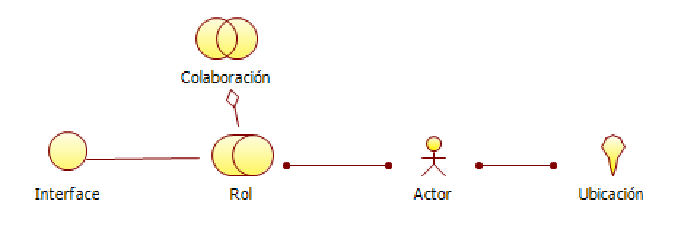
\includegraphics[width=1.0\textwidth]{Arquitectura/images/modelo/Punto_de_Vista_de_Organizacion.pdf}
        \caption{Modelo Punto de Vista Organizacional. . Fuente original}
    \end{figure}
\newpage
\subsubsection{Ejemplo}
    \begin{figure}[th!]
        \centering
        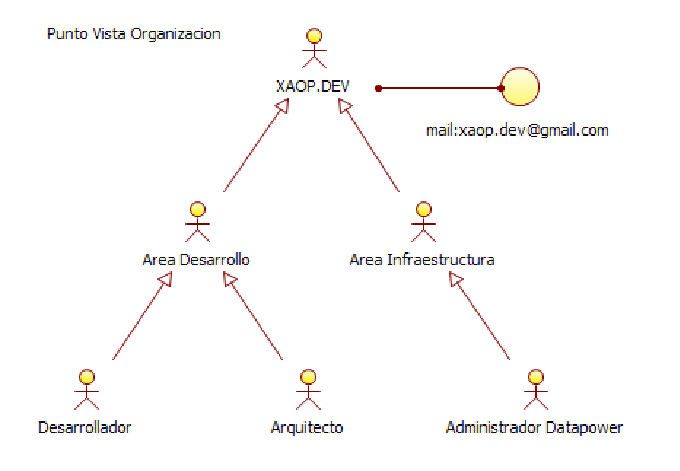
\includegraphics[width=1.0\textwidth]{Arquitectura/images/Punto_de_Vista_de_Organizacion.pdf}
        \caption{Ejemplo Punto de Vista Organizacional.}
    \end{figure}
\newpage

\subsection{Punto de Vista Cooperación de Actor}
Este punto de vista se centra en las relaciones de los actores entre si y su entorno. Un ejemplo comun es el diagrama de contexto, lo que pone una organizacion en su entorno, que consiste en las partes externas, tales como clientes, proveedores y otros socios comerciales. Es muy util en la determinacion de las dependientes externas y colaboraciones y mostrar la cadena de valor o de la red en el que opera el actor.
\subsubsection{Modelo}
    \begin{figure}[th!]
        \centering
        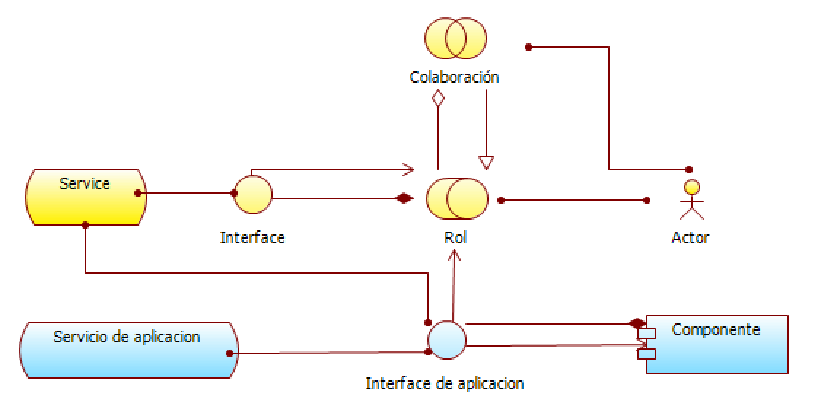
\includegraphics[width=1.0\textwidth]{Arquitectura/images/modelo/Punto_de_Vista_de_Cooperacion.pdf}
        \caption{Modelo Punto de Vista Cooperación de Actor}
    \end{figure}
\newpage
\subsubsection{Ejemplo}
    \begin{figure}[th!]
        \centering
        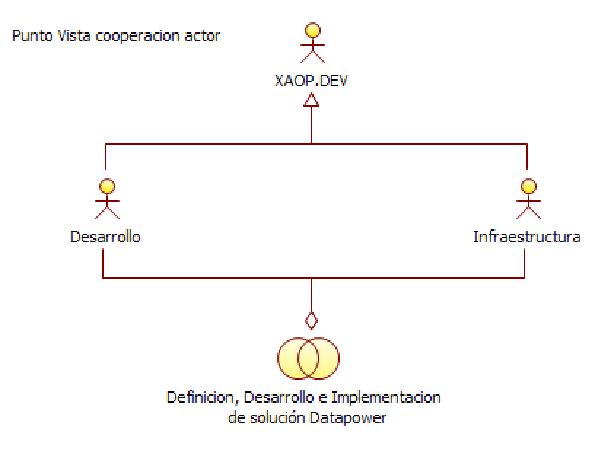
\includegraphics[width=1.0\textwidth]{Arquitectura/images/Punto_de_Vista_de_Cooperacion.pdf}
        \caption{Ejemplo Punto de Vista Cooperación de Actor}
    \end{figure}
\newpage

\subsection{Punto de Vista Función del Negocio}
Muestra las principales funciones de negocio de una organizacion y sus relaciones en terminos de los flujos de informacion, el valor, y cosas entre ellos. Las funciones de la empresa seutilizan para representar los aspectos mas estables de una empresa en terminos de las actividades primarias que realiza, independientemente de los cambios de organizacion o desarrolos tecnologicos.
\subsubsection{Modelo}
    \begin{figure}[th!]
        \centering
        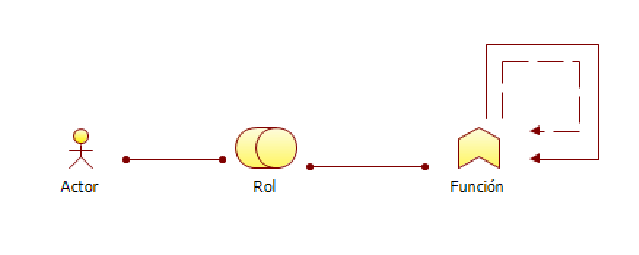
\includegraphics[width=1.0\textwidth]{Arquitectura/images/modelo/Punto_de_Vista_de_Funcion_del_Negocio.pdf}
        \caption{Modelo Punto de Vista Funcion del Negocio}
    \end{figure}
\newpage
\subsubsection{Ejemplo}
    \begin{figure}[th!]
        \centering
        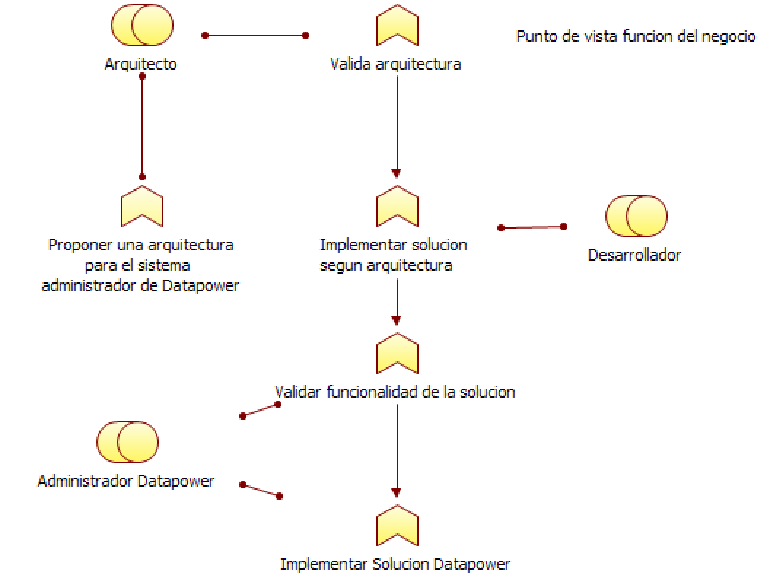
\includegraphics[width=1.0\textwidth]{Arquitectura/images/Punto_de_Vista_de_Funcion_del_Negocio.pdf}
        \caption{Ejemplo Punto de Vista Funcion del Negocio}
    \end{figure}
\newpage

\subsection{Punto de Vista Proceso del Negocio}
Se utiliza para mostrar la estructura de alto nuvel y la composicion de un o mas procesos de negocio.
\subsubsection{Modelo}
    \begin{figure}[th!]
        \centering
        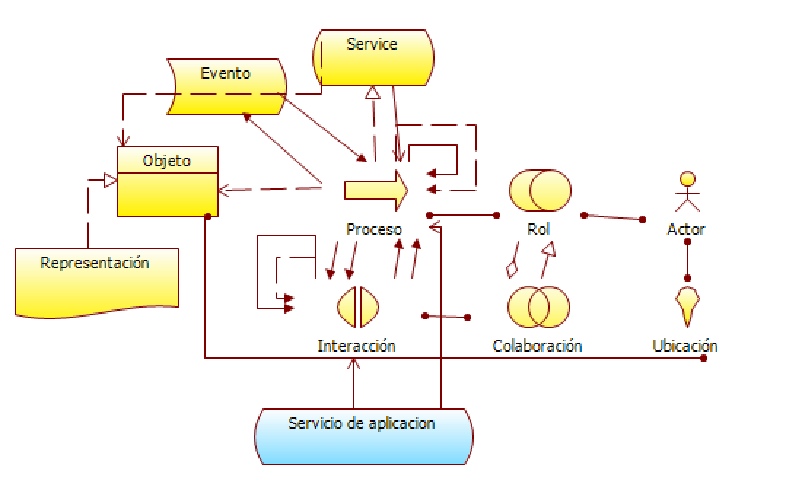
\includegraphics[width=1.0\textwidth]{Arquitectura/images/modelo/Punto_de_Vista_de_Proceso_de_Negocio.pdf}
        \caption{Modelo Punto de Vista Proceso del Negocio}
    \end{figure}
\newpage
\subsubsection{Ejemplo}
    \begin{figure}[th!]
        \centering
        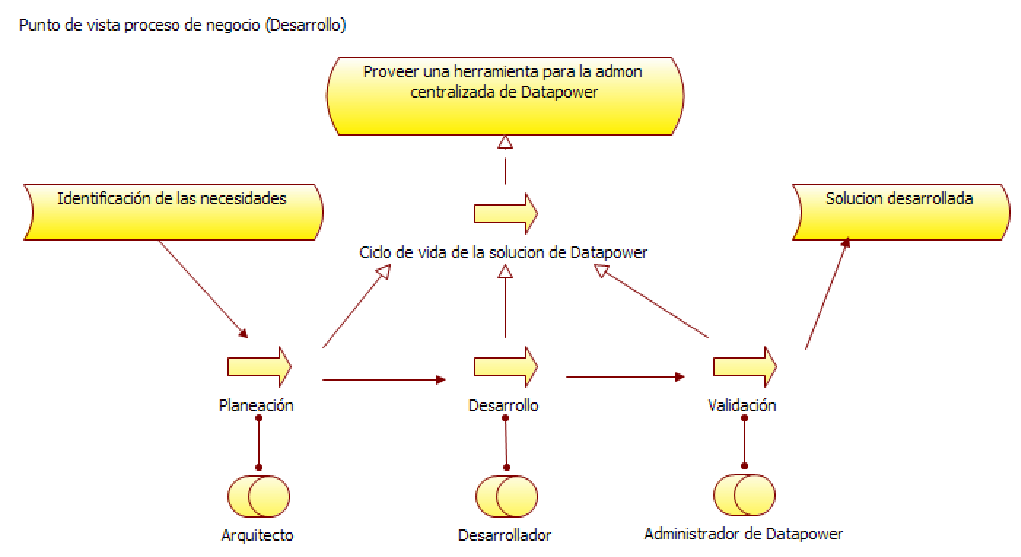
\includegraphics[width=1.0\textwidth]{Arquitectura/images/Punto_de_Vista_de_Proceso_de_Negocio_Desarrollo.pdf}
        \caption{Ejemplo Punto de Vista Proceso del Negocio (Desarrollo)}
    \end{figure}
\newpage
\subsubsection{Ejemplo}
    \begin{figure}[th!]
        \centering
        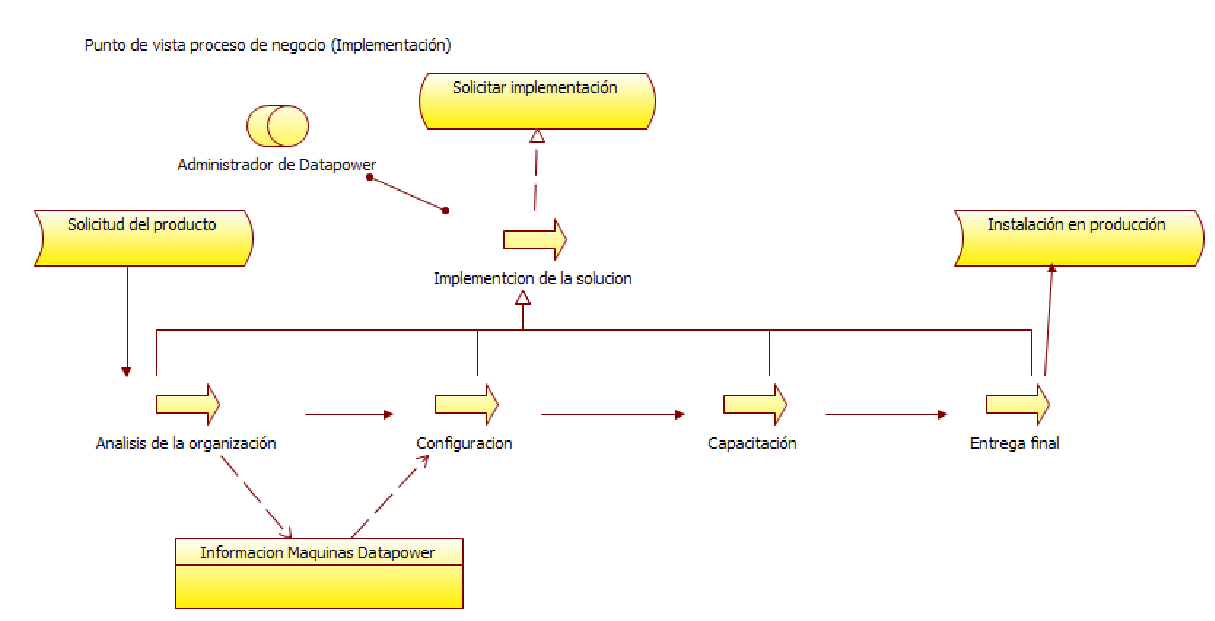
\includegraphics[width=1.0\textwidth]{Arquitectura/images/Punto_de_Vista_de_Proceso_de_Negocio_Implementacion.pdf}
        \caption{Ejemplo Punto de Vista Proceso del Negocio (Implementacion)}
    \end{figure}
\newpage

\subsection{Punto de Vista Producto}
El punto de vista del producto representa el valor que el producto ofrece para los clientes y muestra como esta compuesto el producto que se esta ofreciendo, representa cada uno de los modulos por los que se compone la solución.
\subsubsection{Modelo}
    \begin{figure}[th!]
        \centering
        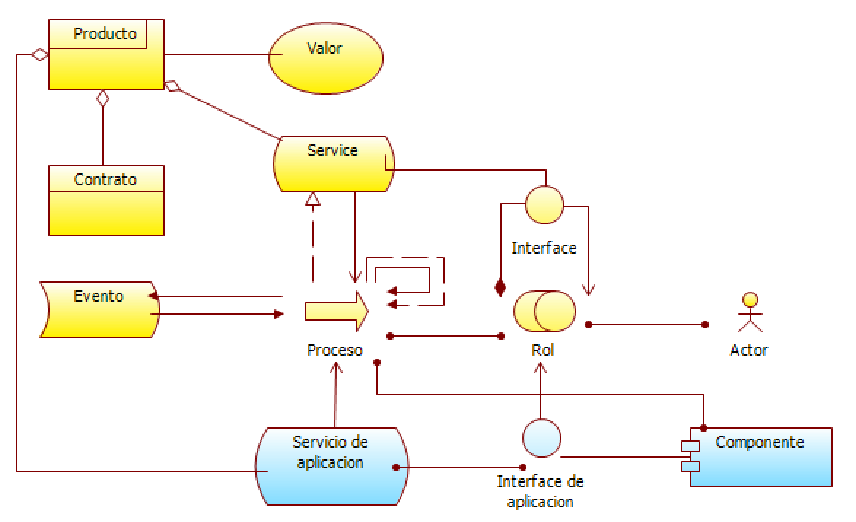
\includegraphics[width=1.0\textwidth]{Arquitectura/images/modelo/Punto_de_vista_Producto.pdf}
        \caption{Modelo Punto de Vista Producto}
    \end{figure}
\newpage
\subsubsection{Ejemplo}
    \begin{figure}[th!]
        \centering
        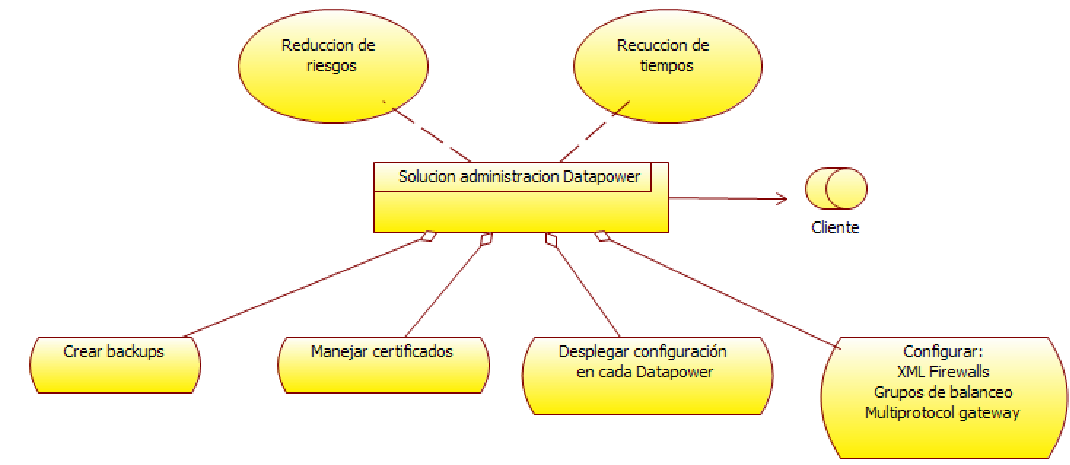
\includegraphics[width=1.0\textwidth]{Arquitectura/images/Punto_de_vista_Producto.pdf}
        \caption{Ejemplo Punto de Vista Producto}
    \end{figure}
\newpage